 \documentclass[11pt,a4paper]{article}
\usepackage[utf8]{inputenc}
\usepackage[finnish]{babel}
\usepackage[T1]{fontenc}
\usepackage{amsmath}
\usepackage{amsfonts}
\usepackage{amssymb}
\usepackage{amsthm}
\pagestyle{plain}
\usepackage{graphicx}
\title{Ketonin suojaus asetaalina}
\author{Delun Li\\014631300\\Orgaanisen kemian työt 1\\Työ 1}
\date{13.10.2018}
\begin{document}

\maketitle

\pagebreak


\section{Johdanto}

Tässä työssä tehtävänä oli suojata ketoniryhmä näytteestämme, etyyliasetoasetaatti, etyleeni asetaalina. Tämän prosessi saavutetaan reagoimalla ketoni etaani-1,2-diolin kanssa happaman katalyytin läsnäollessa. Suojausryhmä, asetaali, poistetaan reagoimalla näyte happaman yhdisteen kanssa, jolloin saadaan suojattu ketoni.$^1$ 

\vspace{0.5cm}

\noindent \textbf{Reaktioyhtälö:}

\vspace{0.3cm}


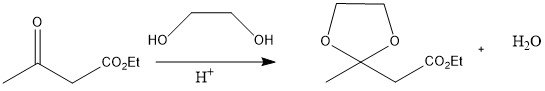
\includegraphics[width=12cm, height=2cm]{yht.jpg}

\vspace{0.3cm}

\noindent Etyyliasetoasetaatin ketoni ryhmä reagoi etaani-1,2-diolin kanssa tolueenisulfonihapon läsnäollessa. Tällöin saadaan tuotteeksi etyyliasetoasetaatti-etyleeniketaali eli fruktoni. Alla on esitetty reaktion mekanismi. 

\noindent \textbf{Reaktion mekanismi:}

\vspace{0.3cm}

\hspace{-1cm}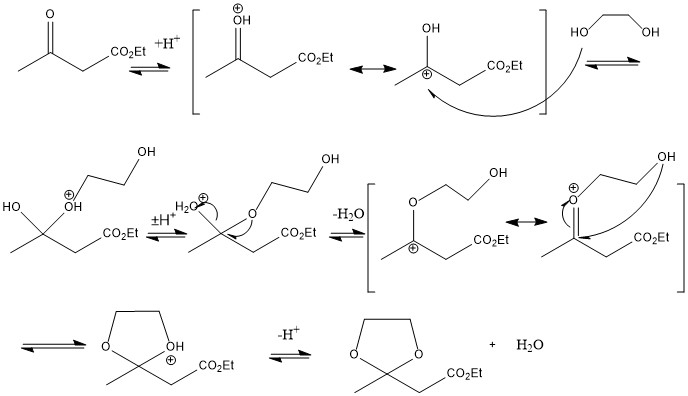
\includegraphics[width=13cm, height=9cm]{mek.jpg}

\vspace{0.3cm}

\noindent Mekanismissa esiintyvä veden poistaminen tapahtuu Dean-Stark laitteistolla, jolloin reaktio painottuu tuotteiden puolelle. 

\section{Työn suoritus}

Kolvi, jossa sisälsi etyyli asetoasetaattia (12,7ml , 0,1003mol), tolueenia (50ml , 0,4721mol), etaani-1,2-diolia (5,8ml , 0,1040mol) ja tolueeni-4-sulfonihappoa (0.054g, 0,0003mol), refluksointiin Dean-Stark laitteistolla. Refluksoidaessa näytettä, erittyy Dean-Stark putkelle kaksi faasikerrosta. Alempi faasikerros oli vettä, jotka taas valutettiin pois. Näytettä refluksoitiin niin kauan kunnes vettä ei enää kertynyt putkeen. Tässä tapauksessa näytettä kiehutettiin noin tunnin verran. Eritettyään vedet pois näytteestä, kolvin annettiin jäähtyä huoneenlämpötilaan. Prosessin nopeuttamiseksi jäähdytettiin kolvia hieman jäähauteessa ja sitten anettiin sen jäähtyä itsekseen huoneenlämpötilaan. 

Kun kolvi laski huoneenlämpötilaan, siirettiin näyte uuttosuppiloon pestäväksi. Näytettä pestiin ensiksi kerran 10$\%$ NaOH:illa (15ml) ja tämän jälkeen kaksi kertaa H$_2$O:lla (20ml). Viimeisen pesun aikana tarkitettiin uutettavan veden pH:ta pH-paperilla. Sillä pH-paperi osoittautui neutraaliksi, niin ei tarvittu uuttaa H$_2$O:lla uudestaan. 

Pesun jälkeen näyte siirettiin erlenmeyerinkolviin kuivattavaksi. Kuivausaineena käytettiin K$_2$SO$_4$. K$_2$SO$_4$ lisättiin sen verran, että ravistettaessa kolvia K$_2$SO$_4$ jauhoa ui liuoksessa. Tässä tapauksessa lisättiin kaksi teelusikallista kuivausainetta. Näytettä kuivattiin yön yli korkki päällä, jottei tuote mahdollisesti haihdu pois. Kuivattuuan, suodatettiin kuivausaineet pois. 

Tämän jälkeen näyte siirettiin rotavaporiin haidutettavaksi, jotta voidaan eristää tolueeni pois näytteestä. Tolueenia haidutettiin näytteestä rotavaporissa 20 minuuttia 50 mbar 40 $^\circ$C:ssa. 


Kun tolueeni on haihtunut pois näytteestä, saadaan haluttu tuote, etyyliasetoasetaatti etyleeni ketaali eli fruktoni. Selvitettiin fruktonin kiehumispiste alipainetislauksella. Tuotetta tislattiin 30 minuuttia ja kihehumispisteeksi saatiin 94$^\circ$C 17,6 mbar:issa. Tämän jälkeen punnittiin tuotteen saanto (8,568g, 50$\%$), taitekerroin (1,4325), IR-spektri ja $^1$H-NMR-spektri.

\section{Johtopäätökset}
 
 Tutkitaan ensiksi liitettä \textbf{IR-spektri}, joka esitettää tuotteen IR-spektriä. Enismmäiseksi huomataan, että spektrissä on erillinen pitkä piikki 1732,60 aallonpituuden kohdalla. Tämä piikki on yhdisteen esteriryhmä. Väliltä 2880-2950 on kolme keskikokoista piikkiä, jotka esittävät yhdisteen sp$^3$ sidoksia CH$_3$ ja CH$_2$. 1040-1190 välillä on kolme vahvaa piikkiä, jotka esittävät yhdisteen etteeriryhmää. Tämän lisäksi 1370:ssa oleva piikki esittää myös CH$_3$ sidosta. $^2$
 
 Liitteessä \textbf{$^1$H-NMR-spektri}:ssä on esitetty tuotteesta saatu $^1$H-NMR spektri. Spektrin 7,25ppm:n kohdalla on käyetyn liuottimen, kloroformin, piikki, jota ei tavitse ottaa tulkinnassa huomioon. Spektristä nähdään, että tuotteen vetysiirtymät ovat pitkälti 1,0-4,5 ppm:n välillä. Välillä 3,8-4,5 ppm ja 1,0-2,0 ppm on kaksi multiplettia. Näiden lisäksi spekrissä on yksi piikki 2,75 ppm:n kohdalla. Liitteessä \textbf{$^1$H-NMR: Tulkinta}:ssa on tulkittu spektriä syvemmin. Ideaalisessa $^1$H-NMR-spektrissä näytteen hiilillä 1 ja 4:llä pitäisi multiplisiteetin olla singletti, 2 ja 3:lla dupletin dupletti, 5:llä quartetti ja 6:lla tripletti. $^{2,3}$
 
 IR-, $^1$H-NMR-spekrin, kiehumispisteen ja taitekertoimen avulla voidaan sanoa, että saatu tuote on selvästi fruktoni. Saatu taitekerroin (1,4325) on hyvin lähellä kirjallisuuden (1,43262) ja myös kiehumispiste (94$^\circ$C 17,6 mbar) on lähellä kirjallisuusarvoa (99,5-101$^\circ$C 17,6mmHg eli $\approx$ 92-94$^\circ$C 17,6mbar).  Arvot olivat kaikki hyvin lähellä kirjallisuusarvoja, jolloin työ on onnistunut hyvin. 
 
 \pagebreak
 
 \section{Viitteet}
 
 \noindent 1. L.M. Harwood, \textit{Experimental Organic Chemistry Principles and Practice}, \textbf{1989}
 
 \noindent 2. Tapio Hase, \textit{Tables For Organic Spectrometry}, \textbf{2008}
 
 \section{Liitteet}
 
 \noindent $^1$H-NMR-spektri
 
 \noindent $^1$H-NMR : Tulkinta
 
 \noindent IR-spektri
 
 \noindent Synteesikaavake.
 
 
 
\end{document}
